% \documentclass{report}
\documentclass[oneside]{memoir}
% \documentclass[preprint,prl,nofootinbib]{revtex4}
% \documentclass[prl]{revtex4-1}

\usepackage{graphicx}% Include figure files
\usepackage{dcolumn}% Align table columns on decimal point
\usepackage{amsmath,amsthm,amssymb,amscd}
\usepackage[utf8]{inputenc}
\usepackage{pstricks}
\usepackage{cite}
\usepackage{verbatim}
% \usepackage[pdftex]{hyperref}


\newcommand{\ra}{\rightarrow}
\newcommand{\xa}{x}
\newcommand{\ta}{t}
\newcommand{\fa}{f}
\newcommand{\D}[1]{\mathcal{D}(#1)}
\newcommand{\LSq}{L^2([0,\pi])}
\newcommand{\R}{\mathbb{R}}
\newcommand{\id}{\text{id}}
\newcommand{\vn}[2]{v_{#1}^{(#2)}}
\newcommand{\wn}[2]{w_{#1}^{(#2)}}
\newcommand{\lb}[2]{\lambda_{#2}^{(#1)}}


\newtheorem{theorem}{Theorem}
\newtheorem{definition}{Definition}
\newtheorem{corollary}{Corollary}
\newtheorem{remark}{Remark}
\newtheorem{conjecture}{Conjecture}


\makechapterstyle{mychapterstyle}{%
  \renewcommand{\chapnamefont}{\LARGE\sffamily\bfseries}%
  \renewcommand{\chapnumfont}{\LARGE\sffamily\bfseries}%
  \renewcommand{\chaptitlefont}{\Huge\sffamily\bfseries}%
  \renewcommand{\printchaptertitle}[1]{%
    \chaptitlefont\hrule height 0.5pt \vspace{1em}%
    {##1}\vspace{1em}\hrule height 0.5pt%
  }%
  \renewcommand{\printchapternum}{%
    \chapnumfont\thechapter%
  }%
}

\chapterstyle{mychapterstyle}
\setsecheadstyle{\Large\sffamily\bfseries}
\setsubsecheadstyle{\large\sffamily\bfseries}
\setsubsubsecheadstyle{\normalfont\sffamily\bfseries}
\setparaheadstyle{\normalfont\sffamily}

\numberwithin{equation}{chapter}
\numberwithin{figure}{chapter}
\numberwithin{table}{chapter}


\setlength{\parindent}{0in}

\begin{document}

\frontmatter

\thispagestyle{empty}

\begin{center}
\large\sffamily Faculty of Physics, Astronomy and Applied Computer Science\\
Jagiellonian University

\vspace*{1cm} {\Huge\sffamily\bfseries Heat flow\\
for harmonic maps between spheres
% on the Outside of the Sphere
\\}
\vspace{2cm}
{\LARGE\sffamily
Paweł Biernat\\
\vspace{3.cm} }
% Faculty of Physics, Astronomy and Applied Computer Science\\
% Jagiellonian University}
% \end{center}

% \begin{center}
% 
\includegraphics[width=0.15\textwidth]{graphics/uj_bw2.eps}
\begin{minipage}{.15\linewidth}
  % LaTeX with PSTricks extensions
%% Creator: inkscape 0.47
%% Please note this file requires PSTricks extensions
\psset{xunit=.05pt,yunit=.05pt,runit=.05pt}
\begin{pspicture}(1092,1755.61572266)
  {
    \newrgbcolor{curcolor}{0 0 0}
    \pscustom[linestyle=none,fillstyle=solid,fillcolor=curcolor]
    {
      \newpath
      \moveto(509.500021,0.49216266)
      \curveto(452.828501,5.10646266)(406.724771,14.84616266)(359.000021,32.28636266)
      \curveto(299.143941,54.15976266)(245.354911,85.27226266)(194.463811,127.45676266)
      \curveto(177.665631,141.38116266)(141.292841,177.73426266)(127.554101,194.33026266)
      \curveto(52.6205,284.84816266)(10.1410996,389.21576266)(1.0145,505.22546266)
      \curveto(0.3559,513.59716266)(0,636.98872266)(0,856.97538266)
      \lineto(0,1195.83016266)
      \lineto(546.000021,1195.83016266)
      \lineto(1091.999971,1195.83016266)
      \lineto(1091.999971,857.58016266)
      \curveto(1091.999971,631.73242266)(1091.648271,514.67796266)(1090.949671,505.33026266)
      \curveto(1082.389971,390.79526266)(1038.785971,283.80546266)(963.986971,193.80566266)
      \curveto(950.407601,177.46666266)(913.928501,141.04126266)(897.540331,127.45676266)
      \curveto(807.345731,52.69276266)(702.546901,9.97186266)(587.054231,0.88816266)
      \curveto(575.038071,-0.05693734)(519.717541,-0.33943734)(509.504121,0.49216266)
      \closepath
      \moveto(598.000021,28.30126266)
      \curveto(684.839321,37.89376266)(760.082561,64.52336266)(830.391721,110.54786266)
      \curveto(861.607681,130.98186266)(886.670161,151.40746266)(913.513741,178.29116266)
      \curveto(940.670081,205.48806266)(961.747731,231.42116266)(982.224611,262.83026266)
      \curveto(1022.516571,324.63346266)(1050.129571,397.51186266)(1060.465671,469.33026266)
      \curveto(1065.704971,505.73456266)(1065.351471,480.88236266)(1065.710671,838.08016266)
      \lineto(1066.043371,1168.83016266)
      \lineto(546.000021,1168.83016266)
      \lineto(25.9566996,1168.83016266)
      \lineto(26.2892996,838.08016266)
      \curveto(26.6483996,480.96196266)(26.2892996,506.01716266)(31.5177,469.33026266)
      \curveto(33.6922,454.06086266)(39.4772,426.09696266)(43.587,410.98956266)
      \curveto(93.4967,227.52096266)(237.861361,86.12096266)(421.500021,40.83706266)
      \curveto(449.125311,34.02486266)(479.512441,29.21326266)(509.500021,26.90266266)
      \curveto(527.141161,25.54346266)(580.695481,26.38976266)(598.000021,28.30126266)
      \closepath
      \moveto(308.887211,181.72876266)
      \curveto(306.900161,182.13686266)(303.729841,183.38216266)(301.842071,184.49596266)
      \curveto(297.585051,187.00766266)(247.901231,225.69356266)(242.706081,230.54166266)
      \curveto(236.759051,236.09146266)(234.563321,241.14126266)(234.536481,249.33026266)
      \curveto(234.509181,257.65106266)(236.680251,262.24036266)(245.947201,273.45066266)
      \curveto(252.344391,281.18946266)(257.475461,284.38546266)(265.203201,285.44466266)
      \curveto(274.486161,286.71696266)(277.794171,284.79126266)(311.479101,258.50496266)
      \curveto(340.143821,236.13626266)(342.669871,233.91466266)(345.291601,228.76756266)
      \curveto(347.572661,224.28936266)(348.125021,221.89046266)(348.125021,216.46246266)
      \curveto(348.125021,208.17806266)(346.258281,204.04466266)(338.063511,194.18426266)
      \curveto(329.539441,183.92766266)(319.353001,179.57906266)(308.887211,181.72876266)
      \closepath
      \moveto(770.154191,182.38876266)
      \curveto(763.040131,184.31776266)(758.665881,187.64626266)(751.705231,196.42686266)
      \curveto(744.662791,205.31076266)(742.547521,210.90346266)(743.259631,218.75666266)
      \curveto(743.887191,225.67746266)(746.542311,231.11126266)(751.665291,235.95896266)
      \curveto(756.825751,240.84226266)(805.325791,278.48376266)(811.046601,282.04556266)
      \curveto(818.952941,286.96816266)(829.332361,286.77646266)(837.065431,281.56516266)
      \curveto(841.813591,278.36536266)(851.813601,266.26786266)(854.618491,260.33026266)
      \curveto(859.036251,250.97846266)(856.842691,237.47446266)(849.882371,231.17366266)
      \curveto(843.222371,225.14476266)(790.087081,184.37786266)(787.500021,183.31226266)
      \curveto(782.376551,181.20176266)(775.818921,180.85266266)(770.154191,182.38876266)
      \closepath
      \moveto(316.583491,266.41796266)
      \curveto(297.360541,281.41286266)(289.180731,288.36406266)(289.809971,289.16986266)
      \curveto(290.671821,290.27366266)(353.444911,370.98296266)(362.850401,383.08026266)
      \curveto(365.309201,386.24276266)(367.523961,388.83026266)(367.772091,388.83026266)
      \curveto(368.477481,388.83026266)(422.945601,346.39306266)(422.974391,345.82106266)
      \curveto(422.988491,345.54096266)(407.647571,325.74096266)(388.883471,301.82106266)
      \curveto(370.119371,277.90116266)(352.403561,255.29186266)(349.515001,251.57836266)
      \lineto(344.263071,244.82646266)
      \lineto(316.583491,266.41796266)
      \closepath
      \moveto(708.112581,294.78836266)
      \curveto(686.600671,322.23906266)(669.000021,345.12956266)(669.000021,345.65626266)
      \curveto(669.000021,346.64046266)(721.190321,387.63986266)(723.316201,388.32576266)
      \curveto(724.432031,388.68576266)(801.245951,290.83836266)(801.723531,288.44866266)
      \curveto(801.919961,287.46576266)(795.180691,282.04666266)(755.903281,251.60416266)
      \lineto(747.225151,244.87806266)
      \lineto(708.112581,294.78836266)
      \closepath
      \moveto(438.702041,347.52886266)
      \curveto(435.237091,348.42796266)(367.551871,401.81606266)(365.689311,405.11916266)
      \curveto(358.572721,417.73976266)(377.835031,439.29086266)(390.315761,432.67186266)
      \curveto(393.222041,431.13056266)(459.160491,379.54676266)(460.893161,377.45906266)
      \curveto(461.637121,376.56256266)(462.474631,373.79916266)(462.754291,371.31796266)
      \curveto(464.210071,358.40236266)(450.199701,344.54526266)(438.702041,347.52886266)
      \closepath
      \moveto(642.491441,348.69526266)
      \curveto(632.249681,353.34796266)(625.359641,367.80236266)(629.703931,375.52176266)
      \curveto(630.691781,377.27706266)(634.875021,381.36006266)(639.000021,384.59506266)
      \curveto(699.526241,432.06266266)(701.934251,433.83026266)(706.074671,433.83026266)
      \curveto(716.541071,433.83026266)(727.000021,422.57796266)(727.000021,411.31756266)
      \curveto(727.000021,408.44656266)(726.351951,405.35006266)(725.495041,404.12666266)
      \curveto(723.854071,401.78376266)(658.069161,350.27776266)(654.000021,348.14996266)
      \curveto(650.600101,346.37196266)(647.256761,346.53036266)(642.491441,348.69526266)
      \closepath
      \moveto(431.294391,413.15596266)
      \curveto(416.331301,424.80186266)(404.068801,434.63116266)(404.044391,434.99886266)
      \curveto(404.019991,435.36656266)(412.908751,447.06656266)(423.797211,460.99886266)
      \curveto(434.685661,474.93116266)(495.739361,553.15526266)(559.472091,634.83022266)
      \curveto(706.777641,823.60570266)(697.138531,811.33016266)(698.065071,811.33016266)
      \curveto(699.743271,811.33016266)(752.908711,769.27178266)(752.551861,768.22648266)
      \curveto(752.344631,767.61948266)(724.768161,732.06952266)(691.270821,689.22652266)
      \curveto(657.773481,646.38352266)(592.213331,562.50526266)(545.581611,502.83026266)
      \curveto(498.949881,443.15526266)(460.279911,393.80186266)(459.648341,393.15596266)
      \curveto(458.775191,392.26306266)(451.980681,397.05576266)(431.294391,413.15596266)
      \closepath
      \moveto(614.319981,415.18826266)
      \curveto(604.320961,427.91636266)(586.203581,450.93026266)(574.059131,466.33026266)
      \curveto(561.914681,481.73026266)(552.095691,494.81896266)(552.239161,495.41616266)
      \curveto(552.553481,496.72466266)(595.286141,551.71646266)(596.000021,551.73116266)
      \curveto(596.275021,551.74116266)(615.069211,528.02386266)(637.764881,499.03586266)
      \curveto(660.460561,470.04776266)(681.050411,443.78576266)(683.520101,440.67586266)
      \lineto(688.010451,435.02136266)
      \lineto(661.255241,414.13106266)
      \curveto(646.539871,402.64136266)(634.050021,392.97206266)(633.500021,392.64356266)
      \curveto(632.950021,392.31506266)(624.319001,402.46026266)(614.319981,415.18826266)
      \closepath
      \moveto(420.278031,663.58022266)
      \curveto(379.531411,715.69272266)(344.336111,760.66178266)(342.066231,763.51148266)
      \lineto(337.939191,768.69288266)
      \lineto(364.719611,789.55198266)
      \curveto(379.448831,801.02458266)(392.024421,810.73343266)(392.665351,811.12734266)
      \curveto(393.407931,811.58372266)(400.282291,803.58793266)(411.614611,789.08688266)
      \curveto(437.962741,755.37132266)(490.227181,688.39552266)(516.265601,654.97892266)
      \curveto(528.844481,638.83582266)(538.919971,625.06402266)(538.655581,624.37502266)
      \curveto(537.893111,622.38802266)(495.875821,568.83026266)(495.079471,568.83026266)
      \curveto(494.685291,568.83026266)(461.024651,611.46776266)(420.278031,663.58022266)
      \closepath
      \moveto(313.000021,770.94678266)
      \curveto(309.421541,772.36368266)(303.170871,778.67048266)(300.810331,783.24608266)
      \curveto(298.011761,788.67068266)(297.912831,795.89068266)(300.587931,799.47728266)
      \curveto(301.736281,801.01688266)(318.082021,814.31196266)(336.911801,829.02190266)
      \curveto(373.005171,857.21828266)(374.851241,858.33138266)(381.266691,855.76612266)
      \curveto(394.897171,850.31589266)(402.203411,831.45433266)(393.443771,824.33016266)
      \curveto(383.875461,816.54831266)(325.922341,771.81938266)(324.315761,770.97638266)
      \curveto(321.692211,769.59968266)(316.437101,769.58588266)(313.000021,770.94638266)
      \closepath
      \moveto(767.000021,771.15768266)
      \curveto(761.072921,774.27598266)(696.876271,825.16878266)(695.491041,827.84753266)
      \curveto(689.478901,839.47372266)(705.663291,859.94446266)(717.931701,856.23149266)
      \curveto(722.128481,854.96135266)(790.402471,801.43708266)(791.834271,798.29458266)
      \curveto(798.021671,784.71468266)(779.565371,764.54718266)(767.000021,771.15768266)
      \closepath
      \moveto(297.426771,822.46850266)
      \curveto(283.821641,840.23119266)(268.131141,848.57559266)(246.481001,849.56207266)
      \curveto(233.112741,850.17119266)(226.136571,848.68022266)(214.336891,842.69213266)
      \curveto(209.272561,840.12209266)(205.521681,838.79974266)(204.456001,839.20868266)
      \curveto(203.511231,839.57122266)(195.584951,845.57445266)(186.842031,852.54918266)
      \lineto(170.945831,865.23052266)
      \lineto(173.222931,867.37683266)
      \curveto(174.475331,868.55731266)(193.050021,883.23214266)(214.500021,899.98758266)
      \curveto(235.950021,916.74302266)(272.850021,945.59712266)(296.500021,964.10780266)
      \curveto(320.150021,982.61849266)(339.950021,997.85905266)(340.500021,997.97572266)
      \curveto(342.119561,998.31926266)(359.081321,960.67013266)(358.359101,958.33485266)
      \curveto(358.018111,957.23227266)(356.038131,954.47144266)(353.959131,952.19967266)
      \curveto(342.862341,940.07390266)(337.031491,924.43713266)(337.007571,906.74012266)
      \curveto(336.990771,894.30107266)(343.469361,877.86576266)(353.557291,864.75573266)
      \curveto(356.065431,861.49622266)(357.875361,858.43747266)(357.579351,857.95852266)
      \curveto(357.283341,857.47956266)(346.794401,849.07124266)(334.270591,839.27336266)
      \curveto(321.746771,829.47548266)(309.651351,819.96563266)(307.391871,818.14037266)
      \lineto(303.283731,814.82171266)
      \lineto(297.426771,822.46850266)
      \closepath
      \moveto(761.336741,835.96349266)
      \curveto(746.576541,847.53885266)(734.171241,857.32051266)(733.769391,857.70051266)
      \curveto(733.367541,858.08051266)(735.578371,861.75264266)(738.682341,865.86079266)
      \curveto(744.722231,873.85468266)(751.030861,886.37647266)(752.870811,894.02298266)
      \curveto(753.491881,896.60403266)(754.000021,902.94455266)(754.000021,908.11302266)
      \curveto(754.000021,925.06049266)(748.644841,939.79514266)(738.458371,950.87547266)
      \curveto(735.258291,954.35635266)(732.991311,957.74727266)(732.978971,959.07147266)
      \curveto(732.948871,962.30079266)(750.050671,998.91689266)(751.244451,998.17910266)
      \curveto(754.274621,996.30635266)(919.552011,866.52682266)(919.810981,865.81686266)
      \curveto(920.290851,864.50134266)(887.763431,838.83016266)(885.616701,838.83016266)
      \curveto(884.574191,838.83016266)(881.646451,840.10621266)(879.110621,841.66582266)
      \curveto(870.105091,847.20451266)(863.426901,849.08434266)(850.951951,849.59217266)
      \curveto(841.203931,849.98899266)(838.166451,849.72279266)(831.465291,847.88435266)
      \curveto(815.078401,843.38867266)(805.735941,836.98035266)(793.909861,822.12377266)
      \lineto(788.173451,814.91738266)
      \lineto(761.336741,835.96349266)
      \closepath
      \moveto(119.500021,905.33203266)
      \curveto(77.6529,937.90301266)(73.2898,941.85293266)(77.4116,943.43461266)
      \curveto(78.7396,943.94422266)(114.62213,941.02791266)(129.339761,939.21422266)
      \lineto(134.179491,938.61780266)
      \lineto(133.458961,957.54533266)
      \curveto(132.704581,977.36190266)(133.095111,980.09079266)(136.856231,981.28452266)
      \curveto(137.878321,981.60892266)(146.934101,979.59470266)(156.980191,976.80848266)
      \curveto(167.026291,974.02226266)(175.348451,971.87482266)(175.473881,972.03639266)
      \curveto(175.599311,972.19796266)(171.668071,990.68844266)(166.737771,1013.12633266)
      \curveto(158.114971,1052.36893266)(157.840941,1053.99690266)(159.541801,1055.87633266)
      \curveto(160.514311,1056.95094266)(161.898381,1057.83016266)(162.617521,1057.83016266)
      \curveto(163.336661,1057.83016266)(180.293601,1049.50516266)(200.299601,1039.33016266)
      \curveto(220.305601,1029.15516266)(236.972471,1020.83016266)(237.337091,1020.83016266)
      \curveto(237.701701,1020.83016266)(238.000021,1029.74016266)(238.000021,1040.63016266)
      \curveto(238.000021,1061.73842266)(238.240731,1062.83016266)(242.894651,1062.83016266)
      \curveto(244.266701,1062.83016266)(252.772691,1060.77466266)(261.796851,1058.26239266)
      \curveto(270.821011,1055.75011266)(278.721851,1053.89317266)(279.354271,1054.13586266)
      \curveto(280.030191,1054.39523266)(282.132861,1065.38164266)(284.455771,1080.79107266)
      \curveto(286.629181,1095.20876266)(288.925681,1107.71382266)(289.559111,1108.58009266)
      \curveto(290.192541,1109.44635266)(291.338381,1109.91322266)(292.105411,1109.61757266)
      \curveto(293.202961,1109.19453266)(336.099721,1013.70741266)(337.218761,1009.19637266)
      \curveto(337.533011,1007.92958266)(341.228441,1010.87826266)(239.109051,930.91215266)
      \curveto(198.194011,898.87303266)(164.219011,872.48021266)(163.609051,872.26146266)
      \curveto(162.999081,872.04270266)(143.150021,886.92446266)(119.500021,905.33203266)
      \closepath
      \moveto(841.794471,939.13759266)
      \curveto(794.656421,976.09350266)(755.559431,1006.86215266)(754.912271,1007.51237266)
      \curveto(753.108671,1009.32446266)(797.597091,1109.83016266)(800.202801,1109.83016266)
      \curveto(801.225791,1109.83016266)(802.265551,1109.26766266)(802.513371,1108.58016266)
      \curveto(802.761191,1107.89266266)(804.788641,1095.42609266)(807.018801,1080.87668266)
      \curveto(809.248971,1066.32726266)(811.283591,1054.21326266)(811.540181,1053.95667266)
      \curveto(811.796771,1053.70008266)(819.806761,1055.59165266)(829.340171,1058.16015266)
      \curveto(838.873581,1060.72866266)(847.577331,1062.83016266)(848.681841,1062.83016266)
      \curveto(849.786351,1062.83016266)(851.505821,1061.92873266)(852.502891,1060.82699266)
      \curveto(854.171381,1058.98333266)(854.263131,1057.31114266)(853.655131,1039.82699266)
      \curveto(853.291791,1029.37873266)(853.223121,1020.83016266)(853.502531,1020.83016266)
      \curveto(853.781941,1020.83016266)(870.732511,1029.19352266)(891.170471,1039.41541266)
      \curveto(923.683681,1055.67664266)(928.622361,1057.86763266)(930.665211,1056.93685266)
      \curveto(932.293501,1056.19495266)(933.000391,1055.03440266)(933.001231,1053.10160266)
      \curveto(933.001901,1051.57731266)(929.146791,1032.84777266)(924.434321,1011.48041266)
      \curveto(919.721851,990.11304266)(916.037621,972.45923266)(916.247141,972.24971266)
      \curveto(916.456661,972.04019266)(925.031571,974.18453266)(935.302501,977.01490266)
      \curveto(959.845451,983.77823266)(958.000021,985.27858266)(958.000021,958.56163266)
      \lineto(958.000021,938.60307266)
      \lineto(962.250021,939.18718266)
      \curveto(973.542931,940.73923266)(1012.292701,943.93182266)(1013.626301,943.42007266)
      \curveto(1017.991271,941.74505266)(1013.955201,938.06566266)(971.656391,905.15983266)
      \curveto(948.092391,886.82851266)(928.517391,871.85600266)(928.156391,871.88759266)
      \curveto(927.795391,871.91919266)(888.932521,902.18168266)(841.794471,939.13759266)
      \closepath
      \moveto(307.841891,1228.49758266)
      \lineto(232.183761,1228.84269266)
      \lineto(230.698141,1233.08642266)
      \curveto(229.423141,1236.72855266)(191.776681,1338.33136266)(98.4189,1590.09067466)
      \curveto(85.8083,1624.09776466)(77,1649.27172466)(77,1651.30548466)
      \curveto(77,1655.50399466)(79.6126,1657.28364066)(84.3087,1656.28395066)
      \curveto(86.0639,1655.91029066)(94.25,1652.56281466)(102.5,1648.84511466)
      \curveto(122.401471,1639.87690466)(134.599611,1635.39357466)(150.406981,1631.23729466)
      \curveto(179.990961,1623.45869466)(184.700171,1621.40394466)(193.500021,1612.43467463)
      \curveto(200.115721,1605.69160466)(206.864011,1593.99211466)(207.189741,1588.70085466)
      \curveto(207.303861,1586.84698466)(207.042791,1581.73017466)(206.609581,1577.33017466)
      \curveto(205.728951,1568.38585466)(205.592601,1568.36277466)(212.515481,1578.33017466)
      \curveto(227.181881,1599.44649466)(242.040301,1606.83592466)(270.500021,1607.16720466)
      \curveto(292.675251,1607.42533466)(303.408921,1603.70188466)(315.372241,1591.60125466)
      \curveto(326.828781,1580.01322466)(331.987921,1568.26825466)(331.963711,1553.83016466)
      \curveto(331.937711,1538.31638466)(327.176051,1527.63195466)(313.975711,1513.46774466)
      \curveto(303.814451,1502.56451266)(302.053761,1498.76647266)(304.181331,1492.33995266)
      \curveto(305.355781,1488.79238266)(306.298721,1487.96040266)(312.681491,1484.83995266)
      \curveto(316.630041,1482.90957266)(319.892021,1480.71439266)(319.930341,1479.96179266)
      \curveto(319.968641,1479.20918266)(317.174601,1475.83418266)(313.721321,1472.46179266)
      \curveto(296.985941,1456.11842266)(276.204901,1453.63631266)(261.322171,1466.20317266)
      \curveto(255.394551,1471.20841266)(251.971391,1487.20197266)(253.803811,1501.33016266)
      \curveto(254.891621,1509.71730266)(253.901911,1513.31243466)(249.941261,1515.36054466)
      \curveto(243.318751,1518.78518466)(235.451161,1515.78684466)(231.291961,1508.25331266)
      \curveto(228.125721,1502.51832266)(226.642361,1491.28833266)(227.339441,1478.33016266)
      \curveto(228.512561,1456.52279266)(236.369501,1437.07029266)(250.658731,1420.59540266)
      \curveto(259.704821,1410.16563266)(267.663361,1404.35986266)(277.269851,1401.18252266)
      \curveto(284.700821,1398.72473266)(286.956611,1398.45407266)(300.500021,1398.39528266)
      \curveto(317.574181,1398.32118266)(325.199221,1400.03164266)(334.766051,1406.08199266)
      \curveto(347.459831,1414.10991266)(354.413531,1423.92559266)(355.626191,1435.52765266)
      \lineto(356.256001,1441.55334266)
      \lineto(350.504421,1445.37102266)
      \curveto(339.834461,1452.45334266)(335.484801,1461.44209266)(335.523291,1476.33016266)
      \curveto(335.542891,1483.90127266)(335.961231,1486.22242266)(338.158451,1490.95017266)
      \curveto(343.159831,1501.71162266)(351.299901,1508.15505266)(364.005811,1511.41016266)
      \curveto(379.429771,1515.36159466)(395.596111,1507.45944266)(403.039941,1492.33016266)
      \curveto(405.163241,1488.01464266)(405.496751,1485.96120266)(405.476151,1477.33016266)
      \curveto(405.449351,1466.08843266)(403.570101,1460.58835266)(396.694531,1451.62813266)
      \lineto(393.086461,1446.92609266)
      \lineto(396.553371,1439.99615266)
      \curveto(402.444471,1428.22052266)(410.909351,1422.02363266)(424.006041,1419.89884266)
      \curveto(434.020161,1418.27416266)(453.315411,1418.56765266)(460.936131,1420.46056266)
      \curveto(479.122651,1424.97792266)(494.126161,1437.42681266)(503.024471,1455.38261266)
      \curveto(511.370371,1472.22372266)(514.987991,1496.90055266)(511.558891,1513.59834466)
      \curveto(508.101441,1530.43414466)(501.786901,1545.73965466)(495.366521,1552.84625466)
      \curveto(489.633931,1559.19154466)(481.545341,1560.10275466)(476.422911,1554.98032466)
      \curveto(474.115651,1552.67306466)(473.847131,1551.73369466)(474.238941,1547.33989466)
      \curveto(474.536441,1544.00360466)(475.746251,1540.64719466)(477.860701,1537.29190466)
      \curveto(482.490911,1529.94449466)(483.202681,1521.13687466)(479.771841,1513.64293466)
      \curveto(475.185251,1503.62450266)(466.624421,1497.44257266)(452.244171,1493.76472266)
      \curveto(444.826871,1491.86770266)(427.412571,1491.00913266)(428.217731,1492.58016266)
      \curveto(432.024151,1500.00732266)(433.142881,1503.59694266)(433.142881,1508.38330266)
      \curveto(433.142881,1518.22340466)(428.842031,1524.14686466)(408.537041,1542.27232466)
      \curveto(392.690511,1556.41789466)(386.644041,1564.73585466)(384.059911,1575.94483466)
      \curveto(381.789251,1585.79411466)(383.934231,1600.63467466)(389.246611,1611.83017466)
      \curveto(399.589871,1633.62792466)(429.675261,1646.18580466)(457.500021,1640.31968466)
      \curveto(465.975221,1638.53290466)(482.285321,1630.86929466)(486.735041,1626.58305466)
      \curveto(488.514301,1624.86915466)(490.207661,1623.70448466)(490.498061,1623.99488466)
      \curveto(490.788461,1624.28527466)(489.843721,1627.62952466)(488.398631,1631.42652466)
      \curveto(483.376101,1644.62339466)(484.159611,1660.30876066)(490.493501,1673.36419066)
      \curveto(491.836751,1676.13290066)(498.154261,1685.08784066)(504.532411,1693.26406066)
      \curveto(522.095891,1715.77887266)(525.139961,1720.63964266)(532.622991,1738.11907266)
      \curveto(536.925671,1748.16959266)(541.404841,1754.64269266)(544.614161,1755.44818266)
      \curveto(546.585711,1755.94300266)(547.845071,1755.40318266)(550.321941,1753.00150266)
      \curveto(553.870951,1749.56025266)(554.639051,1748.19782266)(562.311521,1731.73483266)
      \curveto(568.641981,1718.15141266)(571.858421,1713.24576266)(587.557591,1693.23005066)
      \curveto(593.985221,1685.03512066)(600.295201,1676.08017066)(601.579781,1673.33017066)
      \curveto(607.857361,1659.89126066)(608.597331,1644.55346466)(603.601411,1631.42652466)
      \curveto(602.156321,1627.62952466)(601.211581,1624.28527466)(601.501981,1623.99488466)
      \curveto(601.792381,1623.70448466)(603.485741,1624.86915466)(605.265001,1626.58305466)
      \curveto(609.714721,1630.86929466)(626.024821,1638.53290466)(634.500021,1640.31968466)
      \curveto(662.324781,1646.18580466)(692.410171,1633.62792466)(702.753431,1611.83017466)
      \curveto(708.044251,1600.68011466)(710.210711,1585.79074466)(707.961231,1576.03876466)
      \curveto(705.360461,1564.76387466)(698.861611,1555.97072466)(682.000021,1540.91246466)
      \curveto(662.729761,1523.70312466)(658.857161,1518.25987466)(658.857161,1508.38330266)
      \curveto(658.857161,1503.59694266)(659.975891,1500.00732266)(663.782311,1492.58016266)
      \curveto(664.587471,1491.00913266)(647.173171,1491.86770266)(639.755871,1493.76472266)
      \curveto(625.186161,1497.49103266)(616.877971,1503.48650266)(612.237311,1513.62303466)
      \curveto(608.806181,1521.11760466)(609.505701,1529.92309466)(614.117601,1537.29190466)
      \curveto(617.700371,1543.01638466)(618.910151,1549.76106466)(616.995761,1553.33811466)
      \curveto(616.292921,1554.65139466)(613.949991,1556.43326466)(611.789261,1557.29781466)
      \curveto(601.373611,1561.46533466)(592.085031,1551.89435466)(584.638531,1529.32162466)
      \curveto(578.792921,1511.60169266)(577.766081,1499.98837266)(580.535191,1482.91368266)
      \curveto(585.983091,1449.32123266)(603.658601,1427.62394266)(631.479811,1420.37744266)
      \curveto(638.443631,1418.56360266)(658.170171,1418.30504266)(667.994001,1419.89884266)
      \curveto(681.176171,1422.03750266)(689.979001,1428.50266266)(695.581721,1440.16039266)
      \lineto(698.864341,1446.99061266)
      \lineto(695.280891,1451.66039266)
      \curveto(688.430761,1460.58714266)(686.550711,1466.09821266)(686.523891,1477.33016266)
      \curveto(686.495991,1489.02913266)(688.206431,1493.84416266)(695.013651,1501.22912266)
      \curveto(703.505001,1510.44114266)(716.326811,1514.39921466)(727.994231,1511.41016266)
      \curveto(740.700141,1508.15505266)(748.840211,1501.71162266)(753.841591,1490.95017266)
      \curveto(756.038811,1486.22242266)(756.457181,1483.90127266)(756.476751,1476.33016266)
      \curveto(756.515251,1461.44209266)(752.165581,1452.45334266)(741.495621,1445.37102266)
      \lineto(735.744041,1441.55334266)
      \lineto(736.373851,1435.52765266)
      \curveto(737.233001,1427.30773266)(740.705311,1420.28186266)(746.829691,1414.37127266)
      \curveto(758.335261,1403.26735266)(769.083221,1398.87054266)(786.640891,1398.08518266)
      \curveto(806.011211,1397.21874266)(820.003741,1401.07621266)(830.852381,1410.27344266)
      \curveto(851.371731,1427.66930266)(863.218171,1451.51645266)(864.660601,1478.33016266)
      \curveto(865.357681,1491.28833266)(863.874321,1502.51832266)(860.708081,1508.25331266)
      \curveto(856.548881,1515.78684466)(848.681291,1518.78518466)(842.058781,1515.36054466)
      \curveto(837.946371,1513.23393466)(836.985031,1509.49283266)(838.156651,1500.17507266)
      \curveto(839.908541,1486.24231266)(836.597381,1471.20157266)(830.677871,1466.20317266)
      \curveto(815.795141,1453.63631266)(795.014101,1456.11842266)(778.278721,1472.46179266)
      \curveto(774.825441,1475.83418266)(772.000021,1479.22262266)(772.000021,1479.99165266)
      \curveto(772.000021,1480.76067266)(774.168671,1482.23144266)(776.819251,1483.26001266)
      \curveto(783.913031,1486.01280266)(786.996501,1488.86832266)(788.079341,1493.68766266)
      \curveto(789.390191,1499.52182266)(787.347821,1503.86613266)(779.550121,1511.83016266)
      \curveto(766.160481,1525.50541466)(761.080491,1535.67297466)(760.252001,1550.45519466)
      \curveto(759.336231,1566.79483466)(764.223971,1579.08364466)(776.617421,1591.60125466)
      \curveto(788.599971,1603.70385466)(799.330251,1607.42527466)(821.500021,1607.16720466)
      \curveto(849.687461,1606.83909466)(864.196461,1599.84296466)(878.430371,1579.71584466)
      \curveto(886.577861,1568.19506466)(886.302851,1568.30795466)(885.460491,1576.83017466)
      \curveto(884.284911,1588.72355466)(884.683811,1591.43559466)(888.746641,1599.17199466)
      \curveto(896.866121,1614.63305466)(909.040831,1623.12154466)(930.500021,1628.28343466)
      \curveto(952.945531,1633.68257466)(965.850441,1638.17670466)(989.500021,1648.83014466)
      \curveto(997.750021,1652.54653466)(1005.936101,1655.89683066)(1007.691301,1656.27526066)
      \curveto(1012.383601,1657.28692066)(1015.000001,1655.50961466)(1015.000001,1651.31045466)
      \curveto(1015.000001,1649.26358466)(1004.259501,1618.88529466)(988.583891,1576.59564466)
      \curveto(974.055021,1537.39962466)(939.160841,1443.24847266)(911.041261,1367.37086266)
      \curveto(882.921681,1291.49324266)(859.776521,1229.27332266)(859.607571,1229.10437266)
      \curveto(859.127951,1228.62476266)(392.469251,1228.11156266)(307.841891,1228.49758266)
      \closepath
    }
  }
\end{pspicture}

\end{minipage}
% \end{center}
\vspace{3.cm}

% \begin{center}
\begin{minipage}{0.9\textwidth} {\centering\large\sffamily Thesis written under the
    supervision of Prof. dr hab.  Piotr Bizoń, submitted for the
    Master Degree in the Jagiellonian University\\}
\end{minipage}
\end{center}

\begin{center}
\vspace{1.5cm}
{\large\sffamily Cracow, June 2010}
\end{center}

%%% Local Variables:
%%% mode: latex
%%% TeX-master: "master"
%%% End:


\tableofcontents

\newpage

\mainmatter

\chapter{Introduction}
\label{cha:introduction}

Dirichlet energy $E(u)=\frac{1}{2}\int_M \lVert \nabla u\rVert^2 dV_M$
and its stationary points are central parts of many physical
theories. We can generalize the Dirichlet energy to any map between
differentiable manifolds endowed with inner products. Stationary
points of such functional are called harmonic maps in analogy to
harmonic functions, the main matter of this thesis are harmonic maps
between spheres.
\\

There is a powerful method available in the search for critical point
of a functional $E$ called heat flow. The basic idea behind heat flow
is to define a continuous vector field on the domain of a functional,
such that the functional value decreases along its integral
curves. Therefore, starting with any point as an initial state we can
deform it along the vector field to reach a local minimum and thus, a
stationary point. The heat flow realizes this idea by using an inverse
gradient of $E$ as a vector field in which case integral curves are
formally defined as solutions to
\begin{align*}
  \partial_t F=-\delta E(F),\quad F(0)=F_0,
\end{align*}
where $F_0$ is a starting point and $t$ is a parameter along the
integral curve. The name ``heat flow'' is due to the fact that for the
Dirichlet energy of the form $E(u)=\frac{1}{2}\int_M \lVert \nabla
u\rVert^2 dV_M$ the heat flow turns out to be a heat
equation. Proceeding with this analogy we will henceforth refer to the
parameter $t$ as to time. One expects that the flow will
asymptotically converge to the stationary point of $E$ where the
gradient is zero. This approach has been successfully used by Eells
and Sampson \cite{Eells1964} to prove the existence of harmonic maps
to manifolds of non positive sectional curvature.
\\

If there are two local minima of $E$, by the continuity of the vector
field there exist points which do not flow to either of them, which
stands as a heuristic argument in favor of the existence of a
non-trivial saddle point of a functional. There is however a major
flaw in this reasoning -- in some cases the quasilinear parabolic
equations yield singularities in finite time. Actually in the
particular case of the maps between spheres one can prove using a
theorem by Struwe (Theorem \ref{thm:Struwe}) that the solution
to the heat flow will blow up for some finite $t$.\\

In this thesis we analyse possible asymptotic states and the mechanism
of the blow-up produced by the heat flow for maps between
$k$-dimensional spheres. As the existence of harmonic maps between
spheres has been proved by Bizoń and Chmaj \cite{Bizon1997}, and
Corlette and Wald \cite{Corlette2001} we focus on dynamical aspects of
the heat flow such as stability analysis and the blow-up.

We start by defining the Dirichlet Energy and stating some basic facts
about the harmonic maps in general. Next, we present a symmetric
ansatz to reduce the problem of maps between spheres to maps between
$S^1$ and we proceed by analysing the resulting quasilinear parabolic
partial differential equation in one dimension. The stability of
harmonic maps is analysed in section \ref{sec:stab-ground-stat} and
the blow-up mechanism is described in section \ref{sec:blow-up}.

Numerical results on solving the heat flow in the given ansatz are
presented in chapter \ref{cha:numerical-results} to confirm the
analytical results.



%%% Local Variables:
%%% mode: latex
%%% TeX-master: "master"
%%% End:


\chapter{Preliminaries}
\label{cha:preliminaries}

\section*{Preliminaries}


The energy functional for map $f:M\ra N$ between Riemannian manifolds
$(M,g)$ and $(N,h)$ is defined by
\begin{align}\label{eq:En_general}
  E(u)=\frac{1}{2}\int_M h_{AB}(f)\frac{\partial f^A}{\partial
    x^i}\frac{\partial f^B}{\partial x^j}g^{ij}dV_M\ge0
\end{align}
in local coordinates $x^i$ in $M$ and $f^A$ in $N$. In our case
$M=N=S^k$ with $k\ge3$. Now we use the setup from [Bizon] (TODO excuse
such setup and the details of the domain of the functional), which
simplifies \eqref{eq:En_general} to
\begin{align}
  \label{eq:En_Sk}
  E(u)=\frac{1}{2} V(S^{k-1})\int_{-\pi/2}^{\pi/2}
  \left(f'^2+(k-1)\frac{\sin^2f}{\sin^2\psi}\right) \sin^{k-1}\psi
  d\psi.
\end{align}
The term $V(S^{k-1})$ has no qualitative impact on the behaviour of
the system and we shall drop it from now on. Critical points of such
functional are solutions to the corresponding Euler-Lagrange equation
\begin{align}
  \label{eq:f_psi_EL}
  -\frac{\delta E}{\delta f}=\frac{1}{\sin^{k-1}\psi}\left(\sin^{k-1}\psi
    f'\right)'-\frac{(k-1)}{2}\frac{\sin2f}{\sin^2\psi}=0.
\end{align}

This equation has been extensively studied by Bison and Wald and the
solutions are well known with their properties described in
[]. However, we will approach this problem with the means of the
gradient flow by considering the flow
\begin{equation}
  \label{eq:en_flow}
  \begin{split}
    f_t&=-\frac{\delta E}{\delta f}=\frac{1}{\sin^{k-1}\psi}\left(\sin^{k-1}\psi
      f'\right)'-\frac{(k-1)}{2}\frac{\sin2f}{\sin^2\psi}\\
    f\left(t,0\right)&=0\\
    f\left(t,\pi\right)&=\delta\pi\\
    \delta\in{0,1}
  \end{split}
\end{equation}
Such flow is also known as harmonic map flow because stationary points
of it coincide with the harmonic maps as they are solutions of the ODE
\eqref{eq:f_psi_EL}. The choice of $\delta$ reduces the class of
possible stationary points to maps of homotopy degree up to one. Under
evolution according to \eqref{eq:en_flow} the energy decreases
\begin{align}
  \label{eq:en_t}
  E_t(f)&=\lim_{h\ra0}\frac{E(f(t+h))-E(f(t))}{h}\\
  &=\lim_{h\ra0}\frac{E(f+h f_t+\mathcal{O}(h^2))-E(f)}{h}\\
  % =\lim_{h\ra0}\left(\frac{\delta E}{\delta f}(f_t)+\mathcal{O}h\right)\\
  &=\int_{-\pi/2}^{\pi/2}\frac{\delta E}{\delta f}f_t\sin^{k-1}\psi d\psi\\
  &=-\int_{-\pi/2}^{\pi/2}f_t^2\sin^{k-1}\psi d\psi\le0
\end{align}
with $E_t(f)=0$ iff $f_t=0$. On the other hand, $E(f)\ge0$ so for
generic initial data we would expect energy to asymptotically decrease
to one of its local minimas. Such minimas can be located only at
stationary points which are not unstable under linear
perturbation. Due to the existence of conformal Killing field
$K=\sin(\psi)\frac{\partial}{\partial \psi}$ (with $\mathcal{L}_K
g=-2\cos\psi g$ TODO:check) the only local minimas are constant
solutions $f_0=k\pi$. One can show this by analysing the second
variation of the energy along the $v:=\mathcal{L}_K f=\sin\psi
f'(\psi)$ around the critical point
\begin{align}
  \delta^2E(v,v)
  &=\int_{-\pi/2}^{\pi/2}
  \left(
    v'^2+(k-1)\frac{\cos2f}{\sin^2\psi}v^2
  \right)\sin^{k-1}\psi d\psi\\
  &=-\int_{-\pi/2}^{\pi/2}
  \left(\frac{1}{\sin^{k-1}\psi}\left(\sin^{k-1}\psi
      v'\right)'-(k-1)\frac{\cos2f}{\sin^2\psi}v\right)v\sin^{k-1}\psi
  d\psi\\
  &=-\int_{-\pi/2}^{\pi/2}(Lv)(\psi)v(\psi)\sin^{k-1}\psi d\psi
\end{align}
Now from \eqref{eq:strange_variation} for critical points we have
$Lv=(k-2)v$ and thus $\delta^2 E(v,v)\le0$ and the direction
$v=\sin\psi f'(\psi)$ is unstable. This argument works for any
nonconstant $f$ which is the solution to \eqref{eq:f_psi_EL}. For any
constant solution such vector is null and is the trivial solution to
the linearized equation. On the other hand the only constant solutions
to \eqref{eq:f_psi_EL} are $f_0=0$, $\bar{f}_0=\pi$ and $f_e=\pi/2$
($e$ as in \emph{equatorial}) and using the results from the following
sections we claim that $f_0$ and $\bar{f}_0$ are linearly stable but
$f_e$ is of infinite index for $3\le k\le6$, thus for such choice of
$k$ it is the local maximum rather then local minimum.

% Now when we have briefly introduced the possible local attractors we
% shall ask what is their impact on the global dynamics.
% Apart from being linearly stable, $f_0$ and $\bar{f}_0$ are separated
% (TODO: in what sense?) global minimas of energy functional
% ($E(f_0)=E(\bar{f}_0)=0$), so we would expect that for generic initial
% data the solution should fall into one of such attractors. However, we
% shall see that in the phase space there exists the set of solutions
% that fall to neither of the attractors and thus imply the existence of
% nontrivial solution to \eqref{eq:f_psi_EL}.

(TODO: condition for solution to converge to particular constant
solution)
(TODO: is the attraction pool an open set - yes, from continuity?)

%%% Local Variables:
%%% mode: latex
%%% TeX-master: "master"
%%% End:


\section{Harmonic maps for $F:S^k\ra S^k$}
\label{sec:harmonic-maps-skra}

\subsection{General properties}
\label{sec:general-properties}

From now on we shall set both, the domain and target manifolds to
$S^k$. We choose the coordinate frame on the domain sphere as
\begin{align}
  \label{eq:46}
  x^a=(\psi,\theta),
\end{align}
where $\psi\in(0,\pi)$ is the longitudal angle with
south pole at $\psi=0$ and $\theta$ is the set of coordinates on
$S^{k-1}$ -- the equator of $S^k$. Analogously we introduce
coordinates $(\Psi,\Theta)$ on the target sphere in which the map $F$
takes the form
\begin{align}
  \label{eq:47}
  F^A(\psi,\theta)&=(\Psi,\Theta).
\end{align}
The metric tensors for the given coordinate frames are
\begin{align}
  \label{eq:23}
  &\text{domain:}&\quad &ds^2=d\psi^2+\sin^2\psi^2ds^2\big|_{S^{k-1}}\\
  &\text{target:}&\quad &dS^2=d\Psi^2+\sin^2\Psi^2dS^2\big|_{S^{k-1}}.
\end{align}
Solving equations \eqref{eq:31} without any further assumptions
presents an impossible task, we therefore in section
\ref{sec:basic-setup} introduce a simple ansatz. Still without any
simplifications we can state the following.

\begin{theorem}\label{thm:skk-energy-bound}
  For $k\ge3$ and any given map $F:S^k\ra S^k$ there is a map within
  the homotopy class of $F$ of arbitrary small Dirichlet energy.
\end{theorem}

\begin{proof}
  The proof bases on the fact that on any sphere there exists a one
  parameter group of conformal maps, which in the coordinates
  \eqref{eq:46} has the form
  \begin{align}
    \label{eq:10}
    \psi_A=2\arctan(e^A\tan(\psi/2)).
  \end{align}
  The above conformal map can be depicted as dragging the whole sphere
  along the longitudal coordinates in the direction of one of its poles
  (for $A$ large, this would be the north pole). We define the map $F_A$
  to be a composition
  \begin{align}
    \label{eq:11}
    F_A=F\circ\psi_A.
  \end{align}
  Due to the conformal properties of the map $\psi_A$ we obtain the
  following energy density of $F_A$
  \begin{align}
    \label{eq:12}
    e(F_A)_\psi=&e(F)_{\psi_A}\rho_A^2,\\
    \rho_A=&\frac{1}{\cosh A-\cos\psi\sinh A},
  \end{align}
  where $e(F)_\psi$ is the energy density of $F$ at point $\psi$.  The
  map $F$ is regular, and therefore $e(F)_{\psi_A}$ is bounded by its
  maximal value $C(F)=\max_\psi\left(e(F)_\psi\right)$ and we have the
  following bound
  \begin{align}
    \label{eq:13}
    e(F_A)_\psi&\le C(F)\rho_A^2.
  \end{align}
  Assuming $k\ge3$, the Dirichlet energy of $F_A$ can be bounded by
  \begin{align}
    \label{eq:14}
    E(F_A)&=\int_{S^k}e(F_A)dV_{S^k}\\
    &\le C(F)V(S^{k-1})\int_{0}^{\pi}\rho_A^2\sin^{k-1}\psi d\psi\\
    &\le C(F)V(S^{k-1})\max_\psi(\sin^{k-3}\psi)\int_{0}^{\pi}\rho_A^2\sin^2\psi d\psi\\
    &\le C_1(F,k)\frac{1}{1+\cosh A}.
  \end{align}
  which can be made arbitrary small by an appropriate choice of $A$. The
  above bound is not optimal, but is enough for our purposes. As the map
  $\psi_A$ leaves the north and south poles of $S^k$ unchanged, the map
  $F_A$ is of the homotopy class that $F$ and we conclude by the
  following theorem.

\end{proof}



\subsection{Harmonic map ansatz}
\label{sec:basic-setup}

We simplify our problem by assuming that $\Theta=\theta$ and
$\Psi=f(\psi)$ so the map $F$ takes the form
\begin{align}
  \label{eq:24}
  F:(\psi,\theta)\ra(f(\psi),\theta),
\end{align}
which leaves us with one function as a degree of freedom. The given
setup has been introduced in ~\cite{Eells1964} and it consists of the
idea that, after removing the poles, $S^k$ can be treated as
$(0,\pi)\times S^{k-1}$, for which we use remarks \ref{rem:1} and
\ref{rem:2}.\\

For $F$ to be continuous, we require that
\begin{align}
  \label{eq:27}
  \lim_{\psi\ra0}f(\psi)=n\pi\quad\lim_{\psi\ra\pi}f(\psi)=m\pi.
\end{align}
Moreover, closing the domain of $\psi$ will not have any implications
as long as $F$ is regular so we can drop the limits from \eqref{eq:27}
\begin{align}
  \label{eq:1}
  f(0)=n\pi\quad f(\pi)=m\pi.
\end{align}
The number $\lvert n-m\rvert$ stands for the homotopy degree of a
map.\\

The Dirichlet energy of the considered map now has a more transparent
form
\begin{align}
  \label{eq:En_Sk}
  E(f)=\frac{1}{2} V(S^{k-1})\int_{0}^{\pi}
  \left(f'^2+(k-1)\frac{\sin^2f}{\sin^2\psi}\right) \sin^{k-1}\psi
  d\psi.
\end{align}
Where we have changed the argument of $E$ from $F$ to $f$ as
effectively it is a functional of $f$. The term $V(S^{k-1})$ has no
qualitative impact on the behaviour of the system and we shall drop it
from now on. The energy density of \eqref{eq:En_Sk} with the volume
term $V(S^{k-1})$ dropped is
\begin{align}
  \label{eq:35}
  e(f)=\frac{1}{2}\left(f'^2+(k-1)\frac{\sin^2f}{\sin^2\psi}\right).
\end{align}
By the definition \ref{def:regular-map}, the map $f$ is regular if
\begin{align}
  \label{eq:38}
  e(f)=\frac{1}{2}\left(f'^2+(k-1)\frac{\sin^2f}{\sin^2\psi}\right)<\infty.
\end{align}
The Dirichlet energy of $f$ is
\eqref{eq:En_Sk}
\begin{align}
  \label{eq:36}
  E(f)=\int_0^\pi e(f)\sin^{k-1}\psi d\psi\ge0.
\end{align}
The notable fact is the nontrivial $Z_2$ symmetry of the
functional $E(f)$ manifested as the reflection
\begin{align}
  \label{eq:33}
  f&\ra\pi-f,\\
  E(f)&\ra E(\pi-f)=E(f),
\end{align}
leads to the immediate conclusion that every possible critical point
will have its partner of the same homotopy degree% (they will however
% not fulfill our artificial boundary condition $f(0)=0$, but we leave
% this problem until the next sections)
. This does not hold only for the function invariant to
\eqref{eq:33}. The only function such that $f=\pi-f$ is $f_e=\pi/2$,
which corresponds to mapping the whole sphere to an equatorial (hence
index $e$), but by \eqref{eq:27} it is not continuous, so it cannot be
harmonic. The map $f_e$ will however play an important role
later on, and it is analysed in more detail in the appendix.\\

Critical points of $E(f)$ are solutions to the corresponding
Euler-Lagrange equation
\begin{align}
  \label{eq:f_psi_EL}
  \frac{1}{\sin^{k-1}\psi}\left(\sin^{k-1}\psi f'\right)'-\frac{(k-1)}{2}\frac{\sin2f}{\sin^2\psi}=0.
\end{align}
with the boundary values
\begin{align}
  \label{eq:32}
  f(0)=n\pi\quad f(\pi)=m\pi.
\end{align}
The equation \eqref{eq:f_psi_EL} has trivial solutions of homotopy
degree zero and of the form $f=n\pi$ which attains the global energy
minimum. By remark \ref{rem:1}, the identity map $f=\psi+n\pi$ and, by
\eqref{eq:33}, its image $\bar{f}=-\psi+n\pi$ are also solutions but
of the homotopy degree one. These are the only solutions to
\eqref{eq:f_psi_EL} known in the closed form. Because in general, the
symmetry
\begin{align}
  \label{eq:2}
  E(f+n\pi)=E(f)
\end{align}
implies that any stationary point of $E$ can remain stationary after
being translated by $n\pi$ we henceforth drop the inessential
``$+n\pi$'' to simplify the notion of possible solutions.

The solutions to \eqref{eq:f_psi_EL} are analysed in a detailed way in
papers \cite{Corlette2001,Bizon1997}, where for $3\le k\le6$ the
infinite countable family of solutions have been proved to exist, and
some of their important properties have been revealed.\\

\subsection{Family of nontrivial harmonic maps}
\label{sec:solution-family}

The authors of \cite{Bizon1997} have found out that any regular
solution to \eqref{eq:f_psi_EL} will stay inside the box
$[0,\pi]\times[0,\pi]$, which implies that there are no solutions of
homotopy degree higher than one. For $k\ge7$ no solutions apart from
constant and identity ones exist, but for $3\le k\le 7$ there is a
family of solutions, parametrized by their nodal number being the
number of intersections with $\pi/2$. To be consistent with
\cite{Bizon1997} we denote a solution to \eqref{eq:f_psi_EL} as $f_n$,
$n\in\mathbb{N}_0$ with $f_n$ being the map of degree zero for $n$
even, and of degree one for $n$ odd.

The first solution of degree zero is the trivial one, $f_0=0$ and
which is the only constant regular one. Next, corresponding to $n=1$,
is the identity map $f_1=\psi$, which is the representative of the
degree one family. The solutions for $n>1$ have no closed form, but
from \cite{Bizon1997} we know that each $f_n$ has exactly $n$
intersections with $\pi/2$ and $n-1$ extrema (the latter holds for
$n\ge1$). The functions $f_n$ converge in a non-uniform way to the
solution $f_e$ which due to the convention is also denoted as
$f_\infty$. In \cite{Corlette2001} the authors prove that each $f_n$
is of Morse index $n$, thus $f_0$ is the only local minimum of
$E(f)$. (TODO: A few of the first solutions are depicted in the
figure).


%%% Local Variables:
%%% mode: latex
%%% TeX-master: "master"
%%% End:


\chapter{Gradient flow}
\label{cha:gradient-flow}

\section{Heat flow}
\label{sec:gradient-flow}

We can approach the problem of existence and the properties of
critical points of a functional in several ways. For example in one
dimensional case one can prove the existence of solutions to
Euler-Lagrange equations using some ODE techniques, but this rarely
gives insight into the geometry underlying the functional. Another
more sophisticated way is to analyse the level sets of the functional
and use the infinite dimensional variant of the Morse theory to obtain
critical points as it has been done e.g. in
\cite{Corlette2001}. Finally, there is a powerful technique called the
heat flow, which consists of defining the flow, which moves along
the gradient lines of the functional in the direction of
the negative gradient. \\

The intuition behind the heat flow is that, if it exists for all
times, it will push the solution into a minimum of the functional (if
the functional is bounded from below). This approach is especially
useful in finding a harmonic map of a given degree, because the degree
is conserved during the flow.

The formal setup for the heat flow of the Dirichlet energy
\eqref{eq:7} is
\begin{align}
  \label{eq:33}
    \begin{split}
    \partial_t F^A&=-\delta E(F^A)=\tau(F)^A,\\
    F\big|_{t=0}&=F_0
  \end{split}
\end{align}
where
\begin{align}
  \label{eq:34}
  \tau(F)^C=\Delta_g F^C+\Gamma_{AB}^{C}(h)\frac{\partial
    F^A}{\partial x^a}\frac{\partial F^B}{\partial x^b}g^{ab}.
\end{align}
By our assumption on the domain and the target, \eqref{eq:33} is the
set of quasi-linear parabolic PDE's. Using \eqref{eq:33} we get
\begin{align}
  \label{eq:35}
  \frac{dE}{dt}=-\int_M \partial_t F_A\partial_t F_B h^{AB}
  dV_M\le0
\end{align}
with $dE/dt=0$ if and only if $F$ is harmonic. The flow \eqref{eq:33}
therefore reduces the energy and asymptotically tends to a
critical point of $E$.\\

The question if there exists a harmonic map in the same homotopy class
as the initial data $F_0$ is thus reduced to the question of existence
of a solution of \eqref{eq:33} for all $t$ which is non singular as
$t\ra\infty$. This method was used in \cite{Eells1964} to prove
Theorem \ref{thm:Eells-Sampson}, which now can be reformulated in the
following form:

\begin{theorem}[Eells-Sampson \cite{Eells1964}]\label{thm:Eells-Sampson2}
  If $N$ is compact and has non-positive sectional Riemannian
  curvature, then for every $F_0$ the solution to \eqref{eq:33} exists
  for all times and converges to the minimizing harmonic map as
  $t\ra\infty$.
\end{theorem}

Unfortunately the technique of heat flow is not always so successful
-- the solutions to \eqref{eq:33} are not guaranteed to exist for
arbitrary large times. Actually, there is criterion which guarantees
that the solution will cease to exist at some time $T$:

\begin{theorem}[Struwe \cite{Struwe1996}]\label{thm:Struwe}
  For any time $T>0$ there exists a constant $\epsilon=\epsilon(T)>0$
  such that for any map $F_0:M\ra N$ which is not homotopic to a
  constant and satisfies $E(F_0)<\epsilon$ the solution $F$ to
  \eqref{eq:33} must blow up before time $2T$.
\end{theorem}

In the case when $M$ has non-positive Riemannian curvature the theorem
is still true but empty, because within a given homotopy class, the
smooth harmonic map attains the global minimum which is greater than
the constant $\epsilon(T)$, thus no initial data can fulfill the
criterion $E(F_0)<\epsilon$.

\subsection{Heat flow for $S^k\ra S^k$}
\label{sec:gradient-flow-skra}

From this point we will assume that the map $F:S^k\ra S^k$ satisfies
the ansatz \eqref{eq:18} and we shall consider the functional $E(f)$
as defined in \eqref{eq:21} as a base for \eqref{eq:33}. Applying the
heat flow to \eqref{eq:21} we obtain the following initial
boundary problem

\begin{equation}
  \label{eq:en_flow}
  \begin{split}
    f_t&=\frac{1}{\sin^{k-1}\psi}\left(\sin^{k-1}\psi
      f'\right)'-\frac{(k-1)}{2}\frac{\sin2f}{\sin^2\psi},\\
    f(0,\psi)&=g(\psi),\\
    f(t,0)&=g(0)=0\quad f(t,\pi)=g(\pi)=m\pi.
  \end{split}
\end{equation}

The integer $m$ is equal to the topological degree of the map.  By
\eqref{eq:35} the energy decreases

\begin{align}
  \label{eq:36}
  \frac{dE}{dt}=-\int_0^{\pi}f_t^2\sin^{k-1}\psi d\psi<0
\end{align}

unless $f$ is a stationary point of $E(f)$. By Theorem
\ref{thm:harmonic-map-index} the only point to which the flow can
converge starting from generic initial data is the constant map
$f=n\pi$ for which the energy is zero. The flow will thus reduce the
energy from $E(g)$ to an arbitrary small value. If the initial data is
not homotopic to a constant, Theorem \ref{thm:Struwe} comes into play,
which combined with theorem \ref{thm:harmonic-map-index} guarantees
that the blow-up will occur. Moreover, by the numerical evidence, even
if the boundary values are of the form $g(0)=g(\pi)=0$ the blow-up can
occur if initial data lie in the basin of attraction of $f=\pi$.\\

The flow \eqref{eq:en_flow} conserves the parity of $g$, namely if
\begin{align}
  \label{eq:37}
  g(\psi)=\pm g(\pi-\psi)
\end{align}
then at any given time $t\ge0$ we have
\begin{align}\label{eq:38}
  f(t,\psi)=\pm f(t,\pi-\psi).
\end{align}
Our aim is to make the flow converge to one of the stationary points
of $E$, which we know to have the parity specified by
\eqref{eq:29}. We will henceforth denote by $g_+$ and $g_-$ initial
data obeying
\begin{align}
  \label{eq:39}
  g_+(\psi)&=g_+(\pi-\psi),\quad
  g_-(\psi)&=-g_-(\pi-\psi)
\end{align}
which evolve in the subspaces $H_+$ and $H_-$ defined by

\begin{align}
  \label{eq:40}
  H_\pm=\{f(t,\psi)|\quad f(t,\psi)=\pm f(t,\pi-\psi)\}.
\end{align}

We also remark that

\begin{align}
  \label{eq:41}
  f_{2n}\in H_+,\quad f_{2n+1}\in H_-.
\end{align}

$f_0$ is the global energy minimizer in $H_+$ and $f_1$ is the global
energy minimizer in $H_-$. The energy minimizing property of $f_0$ is
a straightforward, the case of $f_1$ being the energy minimizer for
$H_-$ is not that obvious but follows from the Morse analysis made in
\cite{Corlette2001}. Generic initial data with suitable boundary
conditions in any of those subspaces will converge to one of their
respective ground states unless blow-up occurs. We will discuss the
linear stability of the ground states $f_0$ and $f_1$ in the following
section.

%%% Local Variables:
%%% mode: latex
%%% TeX-master: "master"
%%% End:


\section*{Stability of the ground states}

Given the solution $f_0=0$ we consider the small perturbation of the
form $f=f_0+e^{\lambda t} v$ with $v<<1$. The equation for $v$ is thus
of the form
\begin{align}\label{eq:f0_L}
  v''+(k-1)\cot\psi v'-(k-1)\frac{v}{\sin^2\psi}=\lambda v.
\end{align}
The critical exponents at $\psi=0$ are $1$ and $1-k$. The latter will
be rejected because the finitness of the energy condition yields that
the exponent $\alpha$ at $\psi=0$ has to fulfill
$\alpha>1-\frac{k}{2}$. Now when we know that $v$ and $v'$ are square
integrable we can multiply \eqref{eq:f0_L} by $v\sin^{k-1}\psi$ and
integrate on the interval $[0,\pi]$ to get
\begin{align}
  \lambda\int_0^\pi v^2w d\psi=-\int_0^\pi\left(v'^2+\frac{k-1}{\sin^2\psi}v^2\right)\sin^{k-1}d\psi<0.
\end{align}
All the terms under the integrals are positive for $v\ne0$ so
$\lambda<0$ and $f_0$ is linearly stable.\\

We use the similar reasoning for $f_1=\psi$ to get same critical
exponents and after integration on the interval $[0,\pi/2]$ we obtain
\begin{align}
  \label{eq:f1_lambda}
  \lambda\int_0^{\pi/2} v^2w d\psi=-\int_0^{\pi/2}\left(v'^2+(k-1)\frac{\cos2\psi}{\sin^2\psi}v^2\right)\sin^{k-1}d\psi<0
\end{align}
where we have used the antisymmetry of $v$ during the integration by
parts. This suggests that we could split the phase space into two
subspaces of symmetric and antisymmetric functions with respect to the
point symmetry around $(\psi,f)=(\pi/2,\pi/2)$. Such subspaces are
preserved by \eqref{eq:en_flow}, we shall call them $H^+$ and $H^-$
respectively. However each of $H^+$ and $H^-$ when considered as a
subspace of $H$ has instability due to the Killing field
$K=\sin\psi\frac{\partial}{\partial\psi}$, which is perpendicular to
both of them. (TODO: does $K$ decrease energy for all maps?)

Due to the energy minimizing properties of $f_0$ and $f_1$ we shall
call them the ground states of $H^+$ and $H^-$. (TODO: $f_1$ globally
minimizes the energy for $H^-$).


%%% Local Variables:
%%% mode: latex
%%% TeX-master: "master"
%%% End:


\section*{Blow-up}

As we mentioned, apart from the first global attractor $f_0$ there
exists its image by the reflection symmetry $\bar{f}_0=\pi$ which is
also a global minimum of the energy. It turns out that before reaching
the second attractor the spatial derivative of the solution blows up
at the edges of the interval $[0,\pi]$. As the blow up is localized,
let's say at $\psi=0$, we can rewrite \eqref{eq:en_flow} up to first
corrections in $\psi$
\begin{align}
  \label{eq:2}
  \partial_t h=f''+\frac{(k-1)}{\psi}f'-\frac{k-1}{2}\frac{\sin2h}{\psi^2}.
\end{align}
This equation has the scaling symmetry of the form
$\psi\ra\lambda\psi$ and $t\ra\lambda^2t$ therefore we use the
self-similar ansatz of the form


% We shall now answer the question
% of how the convergence to this attractor is realized for initial data
% $g$ consistent with \eqref{eq:en_flow} for $\delta=0$
% \begin{align}
%   \label{eq:2}
%   f(\psi,0)=g(\psi)\\
%   g(0)=g(\pi)=0.
% \end{align}
% It is clear, that for $g$ close enough to $\pi$ in $L^2([0,\pi])$ the
% solution can have arbitrary small energy and thus should converge to
% $\pi$. However, the boundary conditions prevent the solution from
% converging to $\bar{f}_0$ uniformly,

% First of all, we notice that there exist continous functions $g$ of
% arbitrary small energy, yet close to $\pi$. Such functions are
% obtained by




%%% Local Variables:
%%% mode: latex
%%% TeX-master: "master"
%%% End:


\section{Bisection}
\label{sec:bisection}

% We will now use the gradient flow \eqref{eq:en_flow} to implement the
% dynamical version of simple yet powerful technique called the mountain
% pass, which allows to prove the existence of the saddle point of the
% given functional. The intuition behind this technique is that given
% the path connecting two valleys which are separated by mountains,
% there has to be a point along that path from which if we have dropped
% a ball it won't fall into neither of the valleys, and thus it will has
% to roll down to some saddle point.\\

Although we already know, that $f_2$ and $f_3$ are saddle points of
$E(f)$ we shall demonstrate in this section how to obtain them using
only the gradient flow \eqref{eq:en_flow}.\\

% The implementation of this procedure to $H_+$ will look as follows.
Let us formally denote the basins of attraction of $0$ and $\pi$ as
$\Gamma(0)$ and $\Gamma(\pi)$ respectively. We say formally, because
the solutions to \eqref{eq:en_flow} will blow up (e.g. by Theorem
\ref{thm:Struwe}) before asymptotically converging to either of the
ground states. We start by choosing $g_+\in\Gamma(\pi)\cap H_+$ and
$g_+(0)=g_+(\pi)=0$. We now form a path $g_A\in H_+$ such that
\begin{align}
  \label{eq:93}
  g_A=A\cdot g_+,\quad A\in[0,1].
\end{align}
Obviously for $0\le A\ll1$, $g_A\in \Gamma(0)$, so the curve is hooked
up to both, $\Gamma(0)$ and $\Gamma(\pi)$. As $\Gamma(\pi)$ and
$\Gamma(0)$ are disjoint open sets, the curve leading from one of them
into the another has to contain the closed set which does not belong
to neither of the open sets. By definition, initial data from this set
cannot fall into any of those attractors. This means that there is at
least one $A^*$ such that the flow starting from $g_{A^*}$ is not
going to converge to the global energy minimum. Still, for any initial
data the energy has to decrease along the flow and for $A=A^*$ it
cannot asymptotically decrease to $0$, so its infimum $E^*$ obeys
\begin{align}\label{eq:94}
  E^*=\inf_{t\ge0} E(t)>0
\end{align}
and hence, if $g_{A^*}$ won't blow up, there limiting values are
\begin{align}\label{eq:95}
  \lim_{t\ra\infty}E(t)=E^*>0,\quad \lim_{t\ra\infty}\frac{dE}{dt}(t)=0
\end{align}
but, $dE/dt\ra0$ can happen only if $\partial_t f\ra0$ so
\begin{align}\label{eq:96}
  \lim_{t\ra\infty}f(t,\psi)=f^*(\psi)
\end{align}
which means, that $f^*$ is a symmetric solution to
\eqref{eq:f_psi_EL} with $E(f^*)=E^*$, different from the ground
states and, by construction, it is a saddle point in $H_+$. As $g_+$
was chosen to be generic, by such procedure we will obtain the saddle
point of the lowest index, namely $f^*=f_2$.\\

Analogous procedure can be applied to $H_-$ with $(\psi+g_-)\in
H_-\cap\Gamma(\pi-\psi)$, $g_-(0)=g_-(\pi)=0$ and
\begin{align}
  \label{eq:97}
  g_B=\psi+B\cdot g_-,\quad B\in[0,1]
\end{align}
to obtain $f_3$.\\



%%% Local Variables:
%%% mode: latex
%%% TeX-master: "master"
%%% End:


\chapter{Numerical results}
\label{cha:numerical-results}

\section{Numerical realization of the bisection}
\label{sec:numer-real-mount}

The procedure described in \ref{sec:bisection} can be easily realized
by solving the PDE \eqref{eq:en_flow} numerically. For $H_+$, we start
by choosing $g_+$ to be
\begin{align}
  \label{eq:98}
  g_+(\psi)=\pi\sin\psi.
\end{align}
Then, the proper $A^*$ is found by bisection between the blow-up and
the convergence to $0$. As the bisection cannot yield an exact value
of $A^*$ (due to the finite machine precision) we are not able to
reach precisely the saddle point. Rather, as we are starting a bit off
the mid-line between attractors, the solution slides along it reaching
the neighbourhood of $f_2$ along its stable direction, it stays put
for some time but then starts to move again, slowly decaying along the
unstable direction to finally either fall into $0$ or blow up. The
smaller the numerical error of $A^*$ the closer we get to the mid-line
and the longer solutions stays near $f_2$.\\

From the numerical solutions to PDE \eqref{eq:en_flow} we can read the
quantities involved in approaching and leaving the neighbourhood of
$f_2$. These are the first two modes of $f_2$ along with their
respective eigenvalues as presented in \eqref{eq:69}. To obtain the
eigenvalues $\lb{2}{0}$ and $\lb{2}{2}$ we use the function
$\partial_tf\big|_{r=\pi/2}$ which, while in a close neighbourhood of
$f_2$ is
\begin{align}
  \label{eq:99}
  \partial_t
  f\big|_{r=\pi/2}=-\lambda_0A_0e^{-\lambda_0t}v_0(\pi/2)-\lambda_2A_2e^{-\lambda_2t}v_2(\pi/2)
\end{align}
(we have dropped the upper index for clarity). $v_0(\pi/2)$ and
$v_2(\pi/2)$ are quantities depending on the normalization of our
choice, and to further simplify the calculations we set
\begin{align}
  \label{eq:100}
  v_{0,2}(\pi/2)=1.
\end{align}
The quantities $A_{0,2}$ and $\lb{2}{0,2}$ resulting from fitting the
function \eqref{eq:99} to its analog from numerically solved PDE along
with $A^*$ calculated from the bisection are presented in Table ???.\\

Figures ??? present the stages of the evolution.

% \begin{sideways}
%     \centering
%     \label{fig:Evol2}

% \hspace*{-1.5in}
\begin{figure}[h]
  \label{fig:snapshot2}
  \centering
  \advance\leftskip-3cm
  % GNUPLOT: LaTeX picture with Postscript
\begingroup
  \makeatletter
  \providecommand\color[2][]{%
    \GenericError{(gnuplot) \space\space\space\@spaces}{%
      Package color not loaded in conjunction with
      terminal option `colourtext'%
    }{See the gnuplot documentation for explanation.%
    }{Either use 'blacktext' in gnuplot or load the package
      color.sty in LaTeX.}%
    \renewcommand\color[2][]{}%
  }%
  \providecommand\includegraphics[2][]{%
    \GenericError{(gnuplot) \space\space\space\@spaces}{%
      Package graphicx or graphics not loaded%
    }{See the gnuplot documentation for explanation.%
    }{The gnuplot epslatex terminal needs graphicx.sty or graphics.sty.}%
    \renewcommand\includegraphics[2][]{}%
  }%
  \providecommand\rotatebox[2]{#2}%
  \@ifundefined{ifGPcolor}{%
    \newif\ifGPcolor
    \GPcolortrue
  }{}%
  \@ifundefined{ifGPblacktext}{%
    \newif\ifGPblacktext
    \GPblacktexttrue
  }{}%
  % define a \g@addto@macro without @ in the name:
  \let\gplgaddtomacro\g@addto@macro
  % define empty templates for all commands taking text:
  \gdef\gplbacktext{}%
  \gdef\gplfronttext{}%
  \makeatother
  \ifGPblacktext
    % no textcolor at all
    \def\colorrgb#1{}%
    \def\colorgray#1{}%
  \else
    % gray or color?
    \ifGPcolor
      \def\colorrgb#1{\color[rgb]{#1}}%
      \def\colorgray#1{\color[gray]{#1}}%
      \expandafter\def\csname LTw\endcsname{\color{white}}%
      \expandafter\def\csname LTb\endcsname{\color{black}}%
      \expandafter\def\csname LTa\endcsname{\color{black}}%
      \expandafter\def\csname LT0\endcsname{\color[rgb]{1,0,0}}%
      \expandafter\def\csname LT1\endcsname{\color[rgb]{0,1,0}}%
      \expandafter\def\csname LT2\endcsname{\color[rgb]{0,0,1}}%
      \expandafter\def\csname LT3\endcsname{\color[rgb]{1,0,1}}%
      \expandafter\def\csname LT4\endcsname{\color[rgb]{0,1,1}}%
      \expandafter\def\csname LT5\endcsname{\color[rgb]{1,1,0}}%
      \expandafter\def\csname LT6\endcsname{\color[rgb]{0,0,0}}%
      \expandafter\def\csname LT7\endcsname{\color[rgb]{1,0.3,0}}%
      \expandafter\def\csname LT8\endcsname{\color[rgb]{0.5,0.5,0.5}}%
    \else
      % gray
      \def\colorrgb#1{\color{black}}%
      \def\colorgray#1{\color[gray]{#1}}%
      \expandafter\def\csname LTw\endcsname{\color{white}}%
      \expandafter\def\csname LTb\endcsname{\color{black}}%
      \expandafter\def\csname LTa\endcsname{\color{black}}%
      \expandafter\def\csname LT0\endcsname{\color{black}}%
      \expandafter\def\csname LT1\endcsname{\color{black}}%
      \expandafter\def\csname LT2\endcsname{\color{black}}%
      \expandafter\def\csname LT3\endcsname{\color{black}}%
      \expandafter\def\csname LT4\endcsname{\color{black}}%
      \expandafter\def\csname LT5\endcsname{\color{black}}%
      \expandafter\def\csname LT6\endcsname{\color{black}}%
      \expandafter\def\csname LT7\endcsname{\color{black}}%
      \expandafter\def\csname LT8\endcsname{\color{black}}%
    \fi
  \fi
  \setlength{\unitlength}{0.0500bp}%
  \begin{picture}(10080.00,10080.00)%
      \csname LTb\endcsname%
      \put(5040,9860){\makebox(0,0){\strut{}Asymetric modes of $f_3$ and $f_1$}}%
    \gplgaddtomacro\gplbacktext{%
      \put(2889,6579){\makebox(0,0){\strut{}$t=0.0$}}%
    }%
    \gplgaddtomacro\gplfronttext{%
    }%
    \gplgaddtomacro\gplbacktext{%
      \csname LTb\endcsname%
      \put(2488,8534){\makebox(0,0)[r]{\strut{}$\pi/2$}}%
      \csname LTb\endcsname%
      \put(3157,7777){\makebox(0,0){\strut{}$\pi/2$}}%
    }%
    \gplgaddtomacro\gplfronttext{%
    }%
    \gplgaddtomacro\gplbacktext{%
      \csname LTb\endcsname%
      \put(5577,6579){\makebox(0,0){\strut{}$t=0.5$}}%
    }%
    \gplgaddtomacro\gplfronttext{%
    }%
    \gplgaddtomacro\gplbacktext{%
    }%
    \gplgaddtomacro\gplfronttext{%
    }%
    \gplgaddtomacro\gplbacktext{%
      \csname LTb\endcsname%
      \put(8264,6579){\makebox(0,0){\strut{}$t=1.0$}}%
    }%
    \gplgaddtomacro\gplfronttext{%
    }%
    \gplgaddtomacro\gplbacktext{%
    }%
    \gplgaddtomacro\gplfronttext{%
    }%
    \gplgaddtomacro\gplbacktext{%
      \csname LTb\endcsname%
      \put(2889,3891){\makebox(0,0){\strut{}$t=1.5$}}%
    }%
    \gplgaddtomacro\gplfronttext{%
    }%
    \gplgaddtomacro\gplbacktext{%
    }%
    \gplgaddtomacro\gplfronttext{%
    }%
    \gplgaddtomacro\gplbacktext{%
      \csname LTb\endcsname%
      \put(5577,3891){\makebox(0,0){\strut{}$t=2.0$}}%
    }%
    \gplgaddtomacro\gplfronttext{%
    }%
    \gplgaddtomacro\gplbacktext{%
    }%
    \gplgaddtomacro\gplfronttext{%
    }%
    \gplgaddtomacro\gplbacktext{%
      \csname LTb\endcsname%
      \put(8264,3891){\makebox(0,0){\strut{}$t=2.5$}}%
    }%
    \gplgaddtomacro\gplfronttext{%
    }%
    \gplgaddtomacro\gplbacktext{%
    }%
    \gplgaddtomacro\gplfronttext{%
    }%
    \gplgaddtomacro\gplbacktext{%
      \csname LTb\endcsname%
      \put(876,1008){\makebox(0,0)[r]{\strut{}$10^{-2}$}}%
      \put(876,1680){\makebox(0,0)[r]{\strut{}$10^{-1}$}}%
      \put(876,2351){\makebox(0,0)[r]{\strut{}$10^{0}$}}%
      \put(876,3023){\makebox(0,0)[r]{\strut{}$10^{1}$}}%
      \put(876,3695){\makebox(0,0)[r]{\strut{}$10^{2}$}}%
      \put(1008,788){\makebox(0,0){\strut{}$0$}}%
      \put(2352,788){\makebox(0,0){\strut{}$\pi/4$}}%
      \put(3696,788){\makebox(0,0){\strut{}$\pi/2$}}%
      \put(1008,788){\makebox(0,0){\strut{}}}%
      \put(2352,788){\makebox(0,0){\strut{}}}%
      \put(3696,788){\makebox(0,0){\strut{}}}%
      \put(-17,2351){\rotatebox{90}{\makebox(0,0){\strut{}$f_t(t,r)$}}}%
      \put(2352,458){\makebox(0,0){\strut{}$\psi$}}%
      \put(2889,1203){\makebox(0,0){\strut{}$t=3.0$}}%
    }%
    \gplgaddtomacro\gplfronttext{%
    }%
    \gplgaddtomacro\gplbacktext{%
    }%
    \gplgaddtomacro\gplfronttext{%
    }%
    \gplgaddtomacro\gplbacktext{%
      \csname LTb\endcsname%
      \put(5577,1203){\makebox(0,0){\strut{}$t=3.5$}}%
    }%
    \gplgaddtomacro\gplfronttext{%
    }%
    \gplgaddtomacro\gplbacktext{%
    }%
    \gplgaddtomacro\gplfronttext{%
    }%
    \gplgaddtomacro\gplbacktext{%
      \csname LTb\endcsname%
      \put(8264,1203){\makebox(0,0){\strut{}$t=4.0$}}%
      \put(7190,3158){\makebox(0,0)[l]{\strut{}$\vn{1}{3}$}}%
      \put(6652,2674){\makebox(0,0)[l]{\strut{}$\vn{3}{3}$}}%
    }%
    \gplgaddtomacro\gplfronttext{%
    }%
    \gplgaddtomacro\gplbacktext{%
    }%
    \gplgaddtomacro\gplfronttext{%
    }%
    \gplbacktext
    \put(0,0){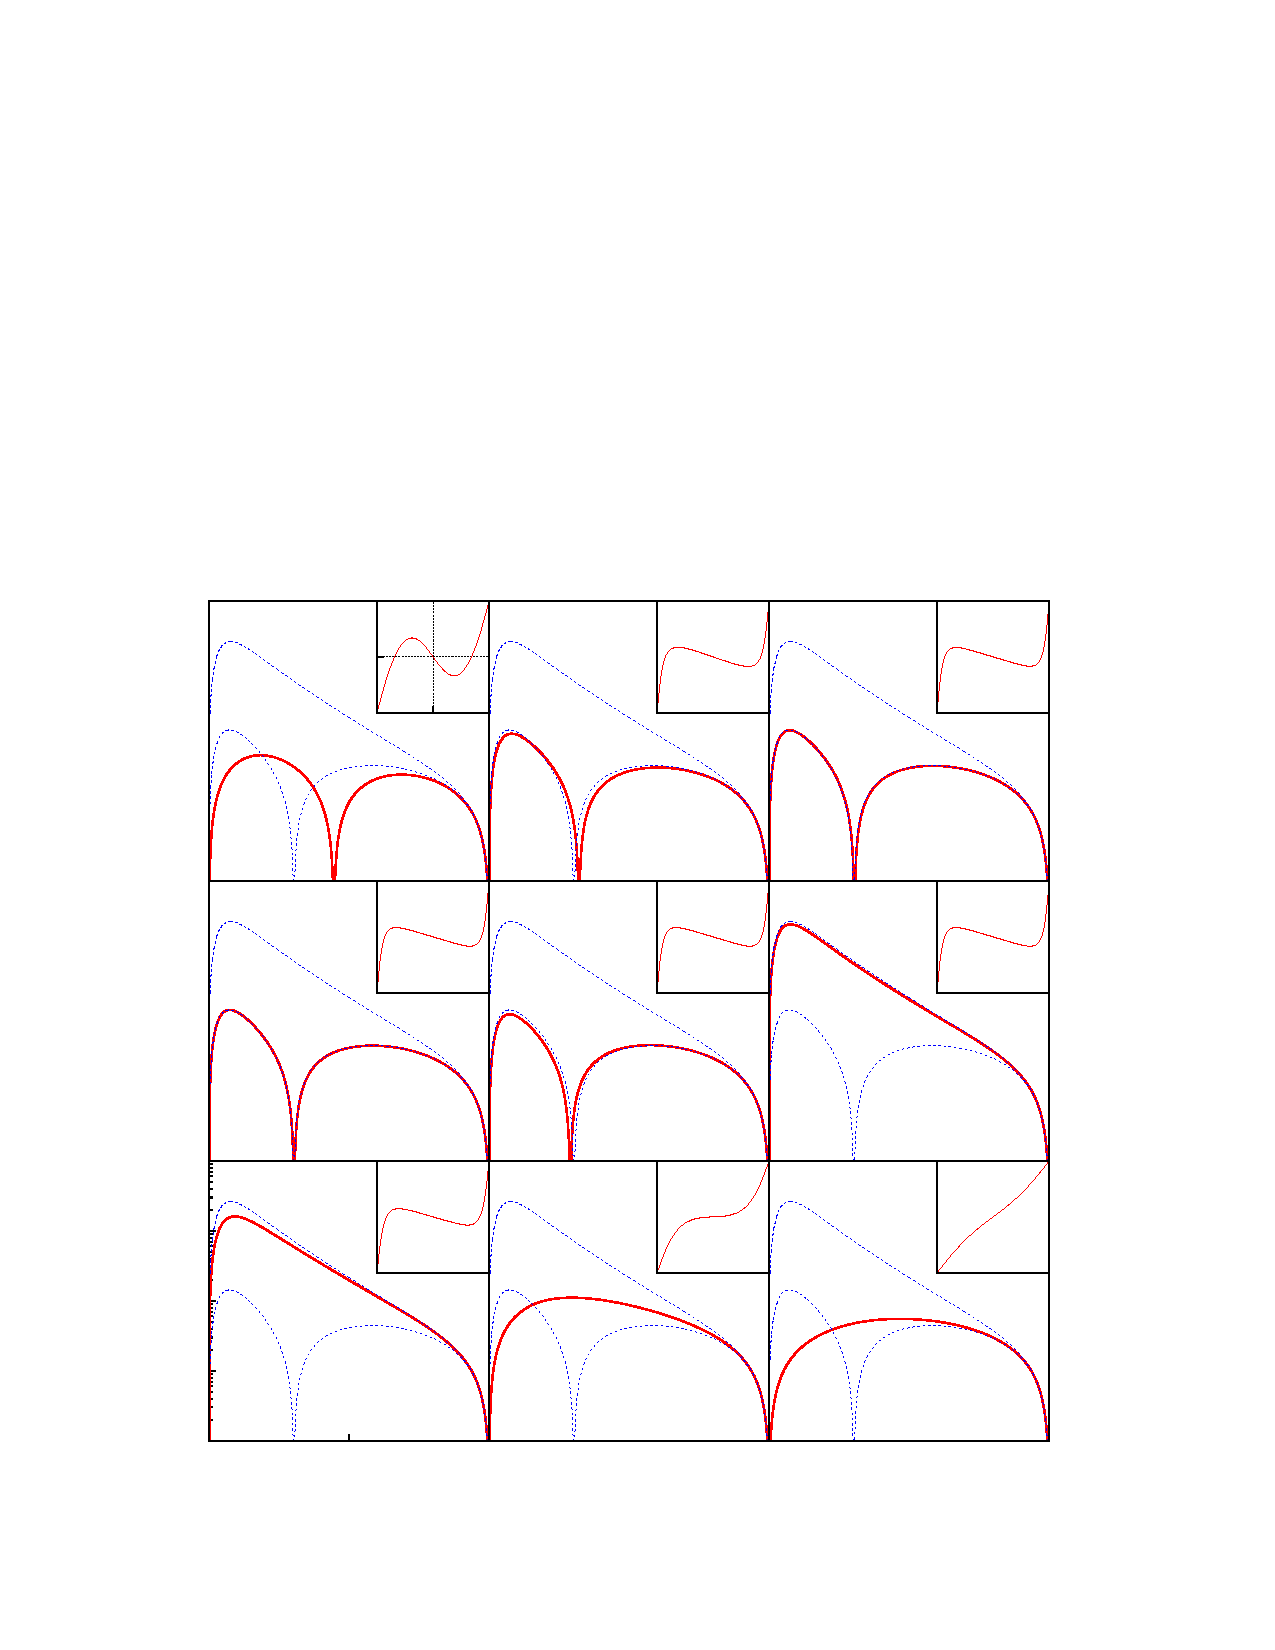
\includegraphics{graphics/snapshot_to_multiplot}}%
    \gplfronttext
  \end{picture}%
\endgroup

  \caption{This figure contains a sequence of snapshots of numerical
    solutions to the gradient flow equation with initial data
    $g_-(\psi)=\psi+B^*\cdot \sin(2\psi)$ with $B^*=...$. Each
    snapshot depicts $\lvert \partial_t f\rvert$ normalized so that
    $\lvert \partial_{tr} f(t,\pi/2)\rvert=1$ along with the plot of
    $f(t)$ in the upper right corner. For comparison the first two
    modes of $f_3$ (blue dashed lines), normalized to
    $v_{1,3}^{(3)\prime}(\pi/2)=1$ have been also depicted. The
    evolution can now be divided into the following stages: ($t=0$)
    non-linear evolution, ($t=1.5-2$) linear convergence to $f_3$
    along $\vn{3}{3}$, ($t=2.5-3.$) linear divergence along
    $\vn{1}{3}$, ($t=3.5$) non-linear approach to ground state $f_1$,
    ($t\ge4$) linear convergence to $f_1$ along $\vn{1}{1}$.}
\end{figure}
    % \caption{The first six non-trivial solutions to}
    %   \eqref{eq:f_psi_EL}}
% \end{sideways}

%%% Local Variables:
%%% mode: latex
%%% TeX-master: "master"
%%% End:


% \chapter{Summary}
\label{cha:summary}


The gradient flow provided us with the means to not only obtain the
unstable harmonic maps between spheres but also allowed the

(in progress)


The results of section \ref{cha:gradient-flow} gave us a
better understanding of what are the possible final states of
evolution under the gradient flow. It has been demonstrated that even
with the possibly singular behaviour, gradient flow can be used as a
tool for determining the possible saddle-type harmonic maps between
spheres by assuming some certain symmetries on the initial
conditions. Still the situation becomes significantly harder if the
stationary points of the
Dirichlet energy is not known a priori.\\



%%% Local Variables:
%%% mode: latex
%%% TeX-master: "master"
%%% End:


\appendix

\clearpage
\chapter{Useful identity}
\label{cha:Identity}

Given the E-L equations
\begin{align}
  \frac{1}{w}\left(wf'\right)'+V(f,x)=0
\end{align}
the second variation in the direction $v=gf'$, for $g$ arbitrary, can
be written as
\begin{align}\label{eq:strange_variation}
  \frac{1}{w}\left(wv'\right)+\frac{\partial V}{\partial
    f}v=\frac{1}{g}\left[\left(\left(\frac{g}{w}\right)'w
  \right)'v-\frac{\partial}{\partial x}\left(g^2 V(f,x)\right)\right]=A(x)v+B(f,x).
\end{align}
Where we have differentiated the E-L equation, multiplied it by $g$
and used the fact that
\begin{align}
  \frac{1}{w}\left(w(gf')'\right)'-g\left(\frac{1}{w}(gf')'\right)'
  =\left(\left(\frac{g}{w}\right)'w \right)'f'-2g'V(f,x).
\end{align}
% In all cases considered in this thesis we have $A(x)=const$ and
% $B(f,x)=0$.
% This cannot be a coincidence and such situation has to
% reflect some particular symmetry of the E-L equation. Worth noticing
% is the fact that in all cases $wg$ is eigenfunction of the laplacian

% \begin{align}
%   \frac{1}{w}\left(w(wg)'\right)'=\lambda wg
% \end{align}

% to some particular $\lambda$ which is also the eigenvalue of the first
% perturbation operator. Moreover $B=0$ implies that
% $V(f,x)=U(f)/g^2(x)$.

\chapter{Numerical methods}
\label{cha:numerical-methods}

\section{Method of lines}
\label{sec:method-lines}

In order to solve the Cauchy problem
\begin{align}
  \label{eq:118}
  \partial_t f=\tau(f),\quad f(0,\psi)=g(\psi)
\end{align}
we discretize the spatial domain in a uniform way to create the grid
of $N$ points
\begin{align}
  \label{eq:107}
  \psi_i=\frac{i-1}{N-1}\pi\in[0,\pi],\quad i\in{1,\dots,N}.
\end{align}
To each point we assign a function of time $f_i(t)$, and we denote the
set of $f_i$ as a vector $\vec{f}\in\mathbb{R}^N$. Then, the solution
to \eqref{eq:118} at points $\psi_i$ can be approximated by $f_i(t)$
if $\vec{f}$ is a solution to the following ordinary differential
equation
\begin{align}
  \label{eq:121}
  \frac{d \vec{f}}{dt}=\hat{\tau}(\vec{f}),\quad f_i(0)=g(\psi_i).
\end{align}
The map $\vec{\tau}:\mathbb{R}^N\ra \mathbb{R}^N$ is a discretized
approximation of $\tau$. As $\tau=\tau(f,\partial_\psi
f,\partial_{\psi\psi} f)$ it is sufficient to choose the
differentiation schemes approximating the first and second
derivatives. We choose the following discretizations of derivatives
called the three point stencil
\begin{align}
  \label{eq:123}
  \partial_\psi f\big|_{\psi_i}\approx D_i\vec{f}=\frac{1}{2h}(f_{i+1}-f_{i-1}),\\
  \partial_{\psi\psi} f\big|_{\psi_i}\approx D_i^2\vec{f}=\frac{1}{h^2}(f_{i+1}-2f_i+f_{i-1}),
\end{align}
where $1\ge i\ge N-1$. We do not define the $D_0$, $D_N$ etc. because
the boundary values imply $df_0/dt=0$ and $df_N/dt=0$ so we don't need
the approximations of $\tau(f)$ at points $\psi_0$ and $\psi_N$. The
above schemes are of order $2$ and $1$ respectively, which means that
\begin{align}
  \label{eq:124}
  \partial_\psi f\big|_{\psi_i}= D_i\vec{f}+\mathcal{O}(h^2),\\
  \partial_{\psi\psi} f\big|_{\psi_i}= D_i^2\vec{f}+\mathcal{O}(h).
\end{align}
With such choice of differentiation schemes we end up with a following
form of \eqref{eq:121}
\begin{align}
  \label{eq:125}
  \frac{d f_i}{dt}=\tau(f_i,D_i\vec{f},D_i^2\vec{f}),\quad f_i(0)=g(\psi_i).
\end{align}
We solve the above equation using a Runge-Kutta method with adaptive
step size described in the next section.

\section{Time marching method}
\label{sec:time-marching-method}

To approximate the solution to the initial value problem for ordinary
differential equation
\begin{align}
  \label{eq:114}
  y'(t)=f(t,y(t)),\quad y(0)=y_0
\end{align}
where $y\in \mathbb{R}^N$ and
$f:\mathbb{R}\times\mathbb{R}^N\ra\mathbb{R}^N$ we use the explicit
Runge-Kutta method with $s$ intermediate steps which approximates
$y_{n+1}=y(t_{n+1})$ by
\begin{align}
  \label{eq:115}
  y_{n+1}=y_n+h\sum_{i=1}^s b_i k_i,
\end{align}
where $k_i$ are the values of the intermediate steps given by
\begin{align}
  \label{eq:117}
  \begin{split}
    k_1 &= f(t_n,y_n), \\
    k_2 &= f(t_n+c_2 h, y_n+a_{21}k_1), \\
    & \ \ \vdots \\
    k_s &= f(t_n+c_s h, y_n + \sum_{j=1}^{s-1} a_{sj}k_j).
  \end{split}
\end{align}
The choice of the constants $c_i$, $a_{ij}$ and $b_i$ uniquely
determines a specific Runge-Kutta (RK) method, there is also a
systematical way of presenting those coefficient called the Butcher's
tableau (table \ref{tab:RKexplicit}).

\begin{table}[h]
  \begin{equation*}
    % \label{eq:19}
    \begin{array}{l | c c c c c}
      \rule{0pt}{2,3ex} 0      \quad &             &               &              &         &   \\
      \rule{0pt}{2,3ex} c_2    \quad & \quad a_{21}  &              &              &         &   \\
      \rule{0pt}{2,3ex} c_3    \quad & \quad a_{31}  & \quad a_{32}  &              &         &   \\
      \rule{0pt}{2,3ex} \vdots \quad & \quad \vdots & \quad \vdots & \quad \ddots &         &   \\
      \rule{0pt}{2,3ex} c_s    \quad & \quad a_{s1}  & \quad a_{s2}  & \quad \cdots & \quad a_{s,s-1} & \\[2,0ex] \hline
      \rule{0pt}{3,3ex}              & \quad b_{1}  & \quad b_{2}    & \quad \cdots & \quad b_{s-1}  & \quad b_{s}
    \end{array}
  \end{equation*}
  \caption{The Butcher tableau for the explicit Runge–Kutta method.}
  \label{tab:RKexplicit}
\end{table}

To calculate the solution in an efficient way one can vary the time
step size $\Delta t_n=t_{n+1}-t_{n}$ to decrease the number of
calculations per a unit of time, keeping the relative error constant
per unit of time. This is realized by combining two $s$-stage RK
methods, one of order $p$ and the other of order $p+1$ which use the
same intermediate values $k_i$, so having the same parameters $c_i$
and $a_{ij}$ but different $b_i$. The solutions are then approximated
by
\begin{align}
  \label{eq:105}
  y_{n+1}=y_n+h\sum_{i=1}^s b_i k_i,\quad y_{n+1}^*=y_n+h\sum_{i=1}^s
  b^*_i k_i,
\end{align}
where stars have been used to denote the coefficients of the method of
order $p+1$. The difference between $y_{n+1}$ and $y_{n}$ gives the
error estimate
\begin{align}
  \label{eq:106}
  \epsilon_i=|(y_{n+1})_i-(y_{n+1}^*)_i|=h\left|\sum_{j=1}^s(b_j-b_j^*)(k_j)_i\right|,\quad
  i\in\{1,\dots,N\}.
\end{align}
If the calculated error or too small compared with the desired error
level the method changes step accordingly to the algorithm described
in \cite{Galassi}. The method of our choice was embedded
Runge–Kutta–Fehlberg (RKF45) of order $4/5$ with the Butcher tableau
presented in table \ref{tab:rkf45}.

\begin{table}[h]
  \centering
  \begin{tabular}{l|lllll}
    0      &           &            &             &           &        \\
    1/4    & 1/4       &            &             &           &        \\
    3/8    & 3/32      & 9/32       &             &           &        \\
    12/13  & 1932/2197 & -7200/2197 & 7296/2197   &           &        \\
    1      & 439/216   & -8         & 3680/513    & -845/4104 &        \\
    1/2    & -8/27     & 2          & -3544/2565  & 1859/4104 & -11/40 \\\hline
    25/216 & 0         & 1408/2565  & 2197/4104   & -1/5      & 0      \\
    16/135 & 0         & 6656/12825 & 28561/56430 & -9/50     & 2/55
  \end{tabular}
  \caption{Butcher tableau for embedded Runge-Kutta-Fahlberg
    method. The lowest row contains $b_i^*$.}
  \label{tab:rkf45}
\end{table}



%%% Local Variables:
%%% mode: latex
%%% TeX-master: "master"
%%% End:


\bibliography{/home/pawel/library.bib}{}
\bibliographystyle{plain}

%%% Local Variables:
%%% mode: latex
%%% TeX-master: "master"
%%% End:



\end{document}

%%% Local Variables:
%%% mode: latex
%%% TeX-master: t
%%% End:
